\documentclass[a4paper,twoside]{report}
\usepackage{geometry}
\usepackage{doc}
\usepackage[latin1]{inputenc}
\usepackage[catalan]{babel}
\usepackage{amsfonts}
\usepackage{amsmath}
\usepackage{graphicx}
\usepackage{listings}
\usepackage{fancyhdr}
\usepackage{fancyvrb}
\usepackage{url} 
\usepackage{color}
\usepackage{lscape}
\usepackage{setspace}

\usepackage[pdfauthor={Ramon Xuriguera Albareda},%
		pdfsubject={BibTeX Bibliography Index Maker},%
		pdftitle={BibTeX Bibliography Index Maker: Meeting notes},%
		pdftex]{hyperref}

\lstset{%
    numbers=none,               %
    breaklines=true,            %
    fancyvrb=false,             %
    tabsize=2,                  % sets default tabsize to 2 spaces
    captionpos=b,               % sets the caption-position to bottom
    frame=single,
    xleftmargin=3em,
    xrightmargin=3em,
    backgroundcolor = \color{lightgrey}
}        


\title{\BibTeX{} Bibliography Index Maker: Meeting Notes}
\author{Ramon Xuriguera}
\date{Primavera 2010}

\setlength{\parindent}{0in}
\definecolor{lightgrey}{gray}{0.85}

%%% PAGE STYLE %%%
\pagestyle{fancy}
\fancyhf{}
\renewcommand{\headrulewidth}{0pt}
\renewcommand{\footrulewidth}{0pt}
\fancyhead[LE]{\textit{\nouppercase{\leftmark}}}
\fancyhead[RO]{\textit{\nouppercase{\rightmark}}}
\fancyfoot[C]{\thepage}
 
\fancypagestyle{plain}{ %
\fancyhf{}
}


\begin{document}
\begin{titlepage}
%\thispagestyle{empty}
\vspace*{44mm}
\hspace{42mm}
\begin{minipage}{112mm}
\textbf{\textit{T�tol:} \BibTeX{} Bibliography Index Maker}\\

\textbf{\textit{Volum:} 1/1}\\
\textbf{\textit{Alumne:} Ramon Xuriguera Albareda}\\

\textbf{\textit{Director/Ponent:} Marta Arias}\\
\textbf{\textit{Departament:} LSI}\\
\textbf{\textit{Data:} Primavera 2010}\\
\end{minipage}

\end{titlepage}

\newpage
\thispagestyle{empty}
\mbox{}

\thispagestyle{empty}
\begin{doublespace}
\hrule
\vspace{5 mm}
\textbf{DADES DEL PROJECTE}
\\
\\
\textit{T�tol del Projecte:}
\\
\\
\textit{Nom de l'estudiant:} Ramon Xuriguera Albareda\\
\textit{Titulaci�:} Enginyeria Inform�tica\\
\textit{Cr�dits:} 37,5\\
\textit{Director/Ponent:} Marta Arias\\
\textit{Departament:} LSI\\
\\
\hrule
\vspace{5 mm}
\textbf{MEMBRES DEL TRIBUNAL} \textit{(nom i signatura)}\\
\\
\textit{President:}
\\
\\
\textit{Vocal:}
\\
\\
\textit{Secretari:}
\\
\\
\hrule
\vspace{5 mm}
\textbf{QUALIFICACI�}
\\
\\
\textit{Qualificaci� num�rica:}\\
\textit{Qualificaci� descriptiva:}
\\
\\
\textit{Data:}\\
\hrule
\end{doublespace}


\tableofcontents

\chapter{Introducci�}
\label{introduction}

\section{Descripci�}
\textit{\BibTeX{} Bibliography Index Maker} �s una eina d'ajuda a la creaci� d'�ndexs bibliogr�fics pensada com un complement a aplicacions de maneig de refer�ncies ja existents com poden ser \textit{\href{http://jabref.sourceforge.net/}{JabRef}}\footnote{\href{http://jabref.sourceforge.net/}{http://jabref.sourceforge.net}} o \textit{\href{http://www.mendeley.com/}{Mendeley}}\footnote{\href{http://www.mendeley.com/}{http://www.mendeley.com}}.

\paragraph{}
La principal funcionalitat consisteix en escanejar un directori que cont� articles cient�fics en PDF i generar un �ndex bibliogr�fic en \BibTeX{} amb les refer�ncies d'aquests fitxers. Aquest �ndex es pot importar des de les aplicacions esmentades o b� pot ser referenciat directament des d'un nou document \TeX.

\section{Treball Existent}
Actualment existeixen nombroses aplicacions dedicades al maneig de refer�ncies. Algunes d'elles utilitzen les meta-dades dels fitxers per tal de trobar informaci� com ara el t�tol o l'autor, per� cap de les eines que hem trobat aprofita el contingut dels documents per generar la refer�ncia.

\paragraph{}
Empreses com ara \textit{Google} o \textit{Microsoft} agafen la informaci� de documents PDF per oferir serveis com ara \textit{Scholar} o \textit{Academic Search}, per� no ofereixen el codi font i per tant, no sabem com funcionen. Per una altra banda, \textit{CiteSeer} �s un projecte \textit{open source} de caracter�stiques similars, per� que tamb� t� limitacions. El sistema funciona analitzant la bibliografia dels articles, informaci� que acostuma a ser bastant estructurada, per� t� problemes per obtenir els camps de la cap�alera del propi fitxer, que �s el que ens interessa.


\chapter{Definici� del Projecte}
\label{definition}
\section{Context}


\section{\BibTeX}
Per poder entendre el context del projecte cal que descrivim l'eina de maneig de refer�ncies \BibTeX i la sintaxi del llenguatge que utilitza. 
En el nostre cas farem servir aquest llenguatge com a format de sortida al generar els �ndexos bibliogr�fics. Al llistat \ref{listing:exampleBibTeX} es mostra un exemple d'una refer�ncia d'un article cient�fic expressat en el format \BibTeX:
\begin{center}
\begin{lstlisting}[caption={Refer�ncia expressada en \BibTeX}, label=listing:exampleBibTeX]
@article{MoSh:27,
  title = {Size direction games over the real line},
  author = {Moran, Gadi and Shelah, M., Saharon},
  journal = {Israel Journal of Mathematics},
  pages = {442--449},
  volume = {14},
  year = {1973},
}
\end{lstlisting}
\end{center}

Alguns aspectes a comentar sobre l'exemple anterior:
\begin{itemize}
\item{}
La primera l�nia cont� el tipus de document i un identificador. El primer defineix els camps obligatoris que s'han d'especificar, i el segon ens permetr� citar a la refer�ncia des d'un document. En el nostre cas nom�s ens interessen les refer�ncies de tipus \textit{article} i haurem de definir, com a m�nim, els camps: \textit{author}, \textit{title}, \textit{journal} i \textit{year}.

\item{}
Es considera que el nom d'un autor o editor pot constar de quatre parts diferents: \textit{First}, \textit{von}, \textit{Last}, \textit{Jr.}. Es poden ordenar de diverses maneres, per� nosaltres ho farem amb \texttt{<von> <last>, <middle>, <first>}. Cal separar m�ltiples noms amb la paraula \texttt{and}.

\item{}
L'�ltim camp d'una refer�ncia pot acabar o no amb una coma.
\end{itemize}

\section{Caracter�stiques}


\section{Planificaci� Temporal}


\chapter{Disseny del sistema}

\section{M�duls}

\chapter{Extracci� dels continguts d'un PDF}
\label{pdftotext}
Un dels aspectes que han influ�t m�s en l'enfocament que hem donat al sistema ha estat la dificultat d'extreure el text dels documents PDF. La primera idea a l'hora d'abordar el nostre projecte va ser intentar extreure informaci� directament dels fitxers PDF dels quals es disposa.

\section{Dificultats}
Les principals dificultats que es troben a l'hora d'obtenir el text d'un fitxer PDF s�n:
\begin{itemize}
\item{Car�cters especials: } com Unicode o lligadures
\item{Flux del text dins del fitxer}
\end{itemize}

\section{Programari existent}
Tot hi haver-hi diverses utilitats que permeten l'extracci� del contingut d'un fitxer PDF en forma de text pla o HTML, totes presenten problemes similars en els punts comentats a la secci� anterior.

A l'ap�ndix \ref{appendix-pdf2text} hi ha exemples de com queden els continguts de diferents documents PDF despr�s d'extreure'ls.


\textbf{xPDF} proporciona eines executables des de la l�nia de comandes per extreure text i altres elements dels fitxers PDF. Es distribueixen binaris de la utilitat tant per Windows com per Linux (que tamb� funcionen per MAC OS).
El principal motiu pel qual hem escollit xPDF �s la qualitat dels resultats, en especial, el fet que no separa els par�grams en diferents l�nies i que obt� el text segons l'ordre de lectura i no l'ordre en que es troben en el document (e.g. dues columnes). Tamb� ser� �til la possibilitat d'extreure les metadades del fitxer de forma f�cil.

Altres opcions que s'han tingut en compte:
\begin{itemize}
\item{PyPDF}
\item{PDFMiner}
\item{PDFBox}
\end{itemize}

 

\chapter{Cerca de refer�ncies a Internet}
\label{ir}


\section{Cercadors}
La primera idea per cercar p�gines que contenen refer�ncies d'art�cles va ser utilitzar \textit{Google Scholar}. La falta d'APIs i el bloqueig peri�dic de les cerques autom�tiques van fer 
Hem preparat el nostre cercador per tal d'utilitzar les APIs dels cercadors \textit{Google}, \textit{Yahoo} i \textit{Bing} i hem 

El principal avantatge �s la 

Un inconvenient, hi ha biblioteques virtuals que no estan indexades en aquests serveis.


\section{Ajustaments}
Podem ajustar la manera com es fan les cerques a partir de certs par�metres que es detallen a continuaci�.

En moltes ocasions, el cercador \textit{Bing} mostra resultats corresponents a \textit{Microsoft Academic Search} (un projecte molt similar a  \textit{Google Scholar}). Aquestes p�gines, per�, no mostren prou informaci� com per generar refer�ncies. Per tant, les hem d'ometre.

\section{\textit{Multithreading}}
Un dels inconvenients m�s grans que implica el fet d'haver d'accedir a Internet, �s que el temps perdut esperant dades �s molt alt. Per reduir-lo, s'ha estudiat la possibilitat d'utilitzar diferents fils d'execuci� per fer m�s d'una consulta de forma m�s o menys simult�nia. La taula seg�ent mostra una comparativa del temps necessari per obtenir m�tliples p�gines web de forma seq�encial o b� utilitzant fins a cinc fils d'execuci� diferents. 

    \begin{center}
    \begin{tabular}{|r|r|r|r|r|r|r|r|}
        \hline
        \multicolumn{2}{|c|}{2 p�gines} & \multicolumn{2}{|c|}{5 p�gines} & \multicolumn{2}{|c|}{10 p�gines} & \multicolumn{2}{|c|}{20 p�gines} \\
        \hline
        Seq. & 5 Threads          & Seq. & 5 Threads          & Seq. & 5 Threads           & Seq. & 5 Threads \\
        \hline
        \hline
        0.9010 & 0.5481 & 2.1830 & 0.6612 & 4.3153 & 1.5914 & 7.9295 & 2.5949 \\
        0.7467 & 0.3795 & 2.1558 & 0.7441 & 4.3186 & 1.2311 & 8.5483 & 2.1958 \\ 
        0.7678 & 0.5641 & 2.0645 & 0.5383 & 9.2930 & 1.4415 & 8.7202 & 2.5749 \\
        0.7421 & 0.3876 & 2.0684 & 0.8551 & 4.9859 & 1.5294 & 8.4732 & 2.2841 \\
        0.9674 & 0.5477 & 2.1510 & 0.8550 & 5.3600 & 1.3116 & 9.2901 & 2.2257 \\
        \hline
        \multicolumn{8}{|l|}{Mitjana:} \\
        \hline
        0.8250 & 0.4854 & 2.1246 & 0.7307 & 5.6546 & 1.4210 & 8.5923 & 2.3751 \\
        \hline
        \multicolumn{8}{|l|}{Guany:} \\
        \hline
        \multicolumn{2}{|c|}{\textbf{-44.96\%}} &  \multicolumn{2}{|c|}{\textbf{-65.6\%}} &  \multicolumn{2}{|c|}{\textbf{-74.87\%}} &  \multicolumn{2}{|c|}{\textbf{-72.35\%}} \\
        \hline
    \end{tabular}
    \end{center}

Les p�gines p�gines corresponen a consultes aleat�ries a Google per evitar l'efecte dels \textit{proxies} i la mem�ria \textit{cache}. Com a conclusi�, tot i que es dades obtingudes no s�n riguroses, ens donen una idea for�a clara de la millora que s'obt� utilitzant aquesta t�cnica.
\paragraph{}
Al nostre sistema hem implementat un \textit{pool} amb un n�mero variable de fils d'execuci� que es van reutilitzant mentre queden refer�ncies per extreure.


\chapter{Extracci� d'Informaci�}
\label{ie}

En aquest cap�tol tractarem

En el nostre context, anomenarem \textit{wrapper} a un tro� de codi que podem utilitzar per extreure una pe�a d'informaci� concreta d'un document.

Podem imaginar-ho com filtre que nom�s ens deixa veure una part del document que ens interessa.

\begin{figure}[h!]
\begin{center}
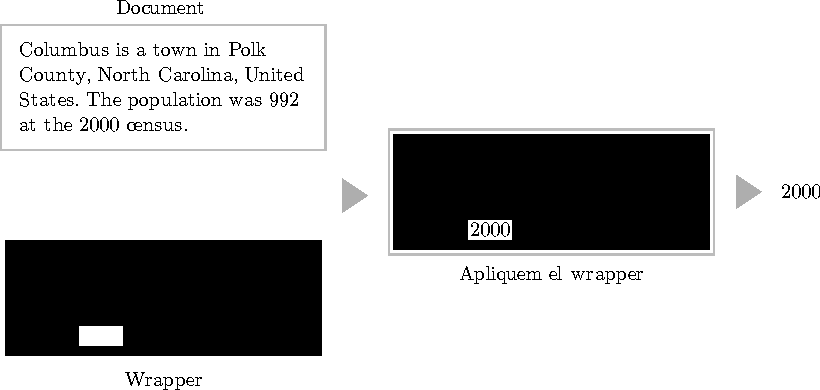
\includegraphics[scale=0.4]{figures/wrapper_sample.pdf}
\end{center}
\end{figure}

\section{\textit{Wrappers} a m�}

\section{Inducci� de \textit{wrappers}}

\subsection{Generaci� autom�tica de regles}
\subsubsection{Ruta d'un element HTML}
\subsubsection{Expressi� regular}

\subsection{Avaluaci� dels \textit{wrappers}}
Una vegada hem generat el conjunt dels \textit{wrappers} possibles per a un conjunt de documents, cal que avaluem quins d'ells funcionen millor. Utilitzem un sistema de vots positius i negatius i en calculem la mitjana amb la seg�ent f�rmula:

\begin{equation*}
    score = \frac{vots\; positius}{vots\; totals}
\end{equation*}

\subsection{Reaprenentatge}
El sistema est� dissenyat per tal que, quan hi ha una davallada en el nombre de refer�ncies extretes correctament, provi de reaprendre els \textit{wrappers} autom�ticament a partir dels exemples que t� emmagatzemats d'execucions passades.

\chapter{An�lisi de resultats}
\label{results}
En aquest cap�tol es mostren les principals proves realitzades amb la nostra aplicaci�. Per cada prova s'explica el perqu� dels resultats obtinguts.

A l'ap�ndix \ref{appendix-results} es mostren tots els test que s'han dut a terme.

\section{Nom�s amb \textit{wrappers} indu�ts}

\section{Utilitzant \textit{wrappers} de refer�ncia}







\chapter{Conclusions i Treball Futur}
\label{conclusions}
\section{Objectius Assolits}

\section{Possibles Millores}


\bibliography{report}
\bibliographystyle{alpha}

\appendix{}
\chapter{Extracci� Contingut PDF}
\label{appendix-pdf2text}

A continuaci� es mostren exemples de com queden les cap�aleres d'alguns fitxers PDF a l'extreure-les en forma de text.

\section{Exemple 01}
\subsubsection{Estructura del PDF}
\begin{figure}[H]
\begin{center}

\includegraphics[width=0.85\textwidth]{figures/pdf2text/pdf2text:01.pdf}
%\caption{Primera idea per l'extracci� de refer�ncies}
\label{fig:pdf2text:01}
\end{center}
\end{figure}

\subsubsection{Text}
Discrete Applied Mathematics 147 (2005) 43 � 55 www.elsevier.com/locate/dam

Pseudo-models and propositional Horn inference
Bernhard Ganter , R�diger Krau�e
Institut f�r Algebra, Technische Universit�t Dresden, Zellescher Weg 12-14, D-01062 Dresden, Germany Received 4 May 2001; received in revised form 6 January 2003; accepted 21 June 2004 Available online 29 December 2004

Abstract A well-known result is that the inference problem for propositional Horn formulae can be solved in linear time. We show that this remains true even in the presence of arbitrary (static) propositional background knowledge. Our main tool is the notion of a cumulated clause, a slight generalization of the usual clauses in Propositional Logic. We show that each propositional theory has a canonical irredundant base of cumulated clauses, and present an algorithm to compute this base. � 2004 Elsevier B.V. All rights reserved.
MSC: 03B05; 03B35; 68T30 Keywords: Horn inference; Horn base; Background knowledge


\section{Exemple 02}
\subsubsection{Estructura del PDF}
\begin{figure}[H]
\begin{center}
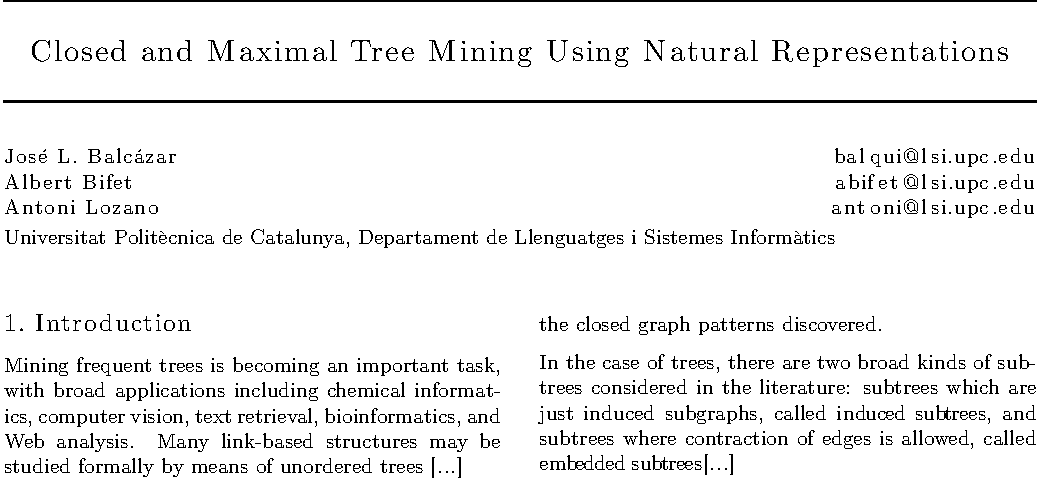
\includegraphics[width=0.85\textwidth]{figures/pdf2text/pdf2text:02.pdf}
\label{fig:pdf2text:02}
\end{center}
\end{figure}

\subsubsection{Text}
Closed and Maximal Tree Mining Using Natural Representations

Jos' L. Balc'zar e a balqui@lsi.upc.edu Albert Bifet abifet@lsi.upc.edu Antoni Lozano antoni@lsi.upc.edu Universitat Polit`cnica de Catalunya, Departament de Llenguatges i Sistemes Inform`tics e a

1. Introduction
Mining frequent trees is becoming an important task, with broad applications including chemical informatics, computer vision, text retrieval, bioinformatics, and Web analysis. Many link-based structures may be studied formally by means of unordered trees.


\section{Exemple 03}
\subsubsection{Estructura del PDF}
\begin{figure}[H]
\begin{center}

\includegraphics[width=0.85\textwidth]{figures/pdf2text/pdf2text:03.pdf}
\label{fig:pdf2text:03}
\end{center}
\end{figure}

\subsubsection{Text}
Applied Economics, 2010, 42, 825�850
\\
\\
Modelling the interactions across international stock, bond and foreign exchange markets\\
Abdul Hakima,* and Michael McAleerb\\
Department of Economics, University of Western Australia, Australia and Faculty of Economics, Indonesian Islamic University, Indonesia b Department of Economics, University of Western Australia, Australia
a
\\
\\
Downloaded By: [Consorci de Biblioteques Universitaries de Catalunya] At: 11:49 20 May 2010\\
\\
The benefits of investing internationally depend on three conditions, namely, cross-country correlations, market volatilities and future changes in currency risks (Odier and Solnik, 1993). This article investigates these conditions for several countries. Many papers have modelled [...]

\chapter{Resultats dels tests}
\label{appendix-results}
A continuaci� es mostren els gr�fics amb la resta de resultats de les proves que s'han realitzat. La majoria corresponen al mateix tipus de tests que els del cap�tol \ref{chapter:results}, per� variant algun par�metre.

\section{Cerca de refer�ncies}
Les gr�fiques seg�ents s�n semblants a la de la figura \ref{fig:results:random-reslen}. En aquest cas, per�, el tipus de fitxers per als quals extraiem consultes i fem les cerques estan agrupats en dues categories segons l'estructura del seu contingut. Per un costat, a la figura \ref{fig:results:pageheader-reslen}, tenim fitxers que tenen una p�gina sencera com a cap�alera abans del resum o \textit{abstract} de l'article.
\begin{figure}[H]
\begin{center}
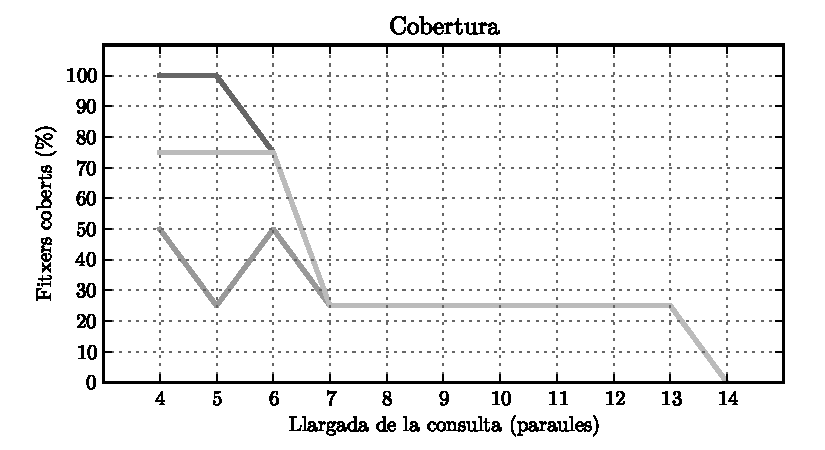
\includegraphics[width=0.8\textwidth]{figures/results:pageheader-reslen.pdf}
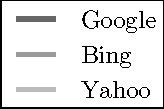
\includegraphics[scale=0.8]{figures/results:search-legend.pdf}
\caption{Qualitat dels resultats per fitxers amb una p�gina sencera com a cap�alera}
\label{fig:results:pageheader-reslen}
\end{center}
\end{figure}

Veiem que per aquest tipus d'article, el percentatge de p�gines per les quals s'han obtingut bons resultats disminueix molt a mesura que s'augmenta la llargada de la consulta. Cal tenir en compte que les consultes s'han obtingut totes a partir de la primera p�gina del fitxer. Al no contenir el resum, fa que l'expressi� regular usada per trobar la consulta no tingui coincid�ncies per la majoria dels articles provats. Si executem les mateixes proves, per� agafant les consultes de les dues primeres p�gines, els resultats milloren for�a:

\begin{figure}[H]
\begin{center}
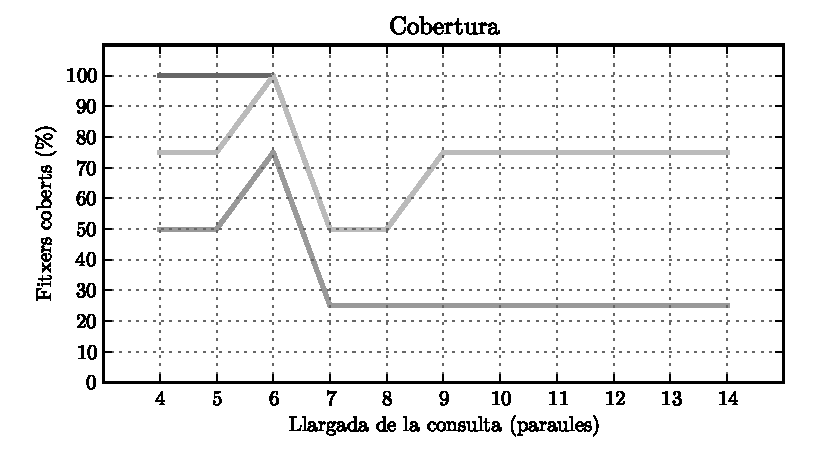
\includegraphics[width=0.8\textwidth]{figures/results:pageheader2-reslen.pdf}
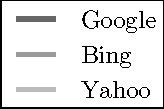
\includegraphics[scale=0.8]{figures/results:search-legend.pdf}
\caption{Qualitat dels resultats per fitxers amb una p�gina sencera com a cap�alera II}
\label{fig:results:pageheader2-reslen}
\end{center}
\end{figure}

El gr�fic de la figura seg�ent s'ha obtingut a partir d'articles que tenen una cap�alera \textit{normal}. Considerem que les cap�aleres dels articles m�s habituals s�n aquelles que tenen l'\textit{abstract} a la mateixa p�gina.
\begin{figure}[H]
\begin{center}
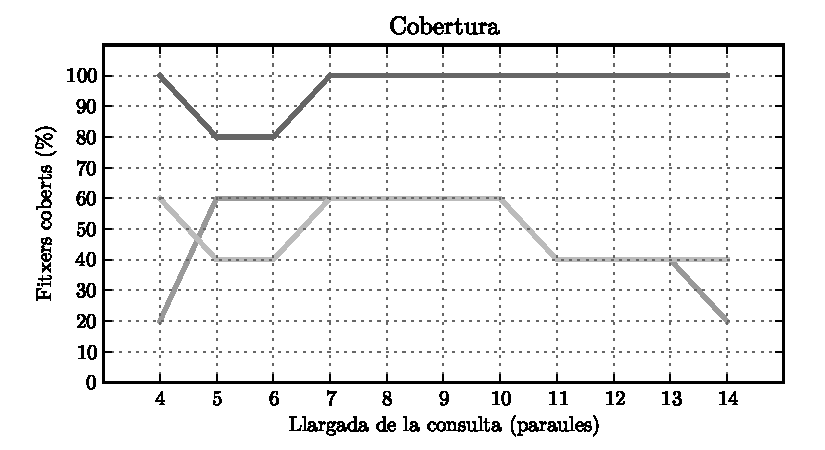
\includegraphics[width=0.8\textwidth]{figures/results:usualheader-reslen.pdf}
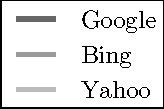
\includegraphics[scale=0.8]{figures/results:search-legend.pdf}
\caption{Qualitat dels resultats per fitxers amb cap�aleres \textit{normals}}
\label{fig:results:usualheader-reslen}
\end{center}
\end{figure}

\paragraph{}
Pel que fa al n�mero de consultes necess�ries per comen�ar a obtenir bons resultats, els gr�fics per aquests dos conjunts de fitxers s�n molt semblants al que hem vist a la figura \ref{fig:results:random-fqlen}.

\section{Generaci� de \textit{wrappers}}
\label{appendix:results:section:wrapperinduction}
Pel que fa a la generaci� autom�tica de regles d'extracci�, la figura seg�ent mostra els \textit{wrappers} obtinguts al generar-los fent servir nom�s dos exemples. Com es pot comprovar,
A continuaci� es mostren els gr�fics de la cobertura dels \textit{wrappers} generats per altres camps que no s'han tractat a la secci� \ref{chapter:results:section:wrapperinduction}.


\begin{figure}[H]
\begin{center}
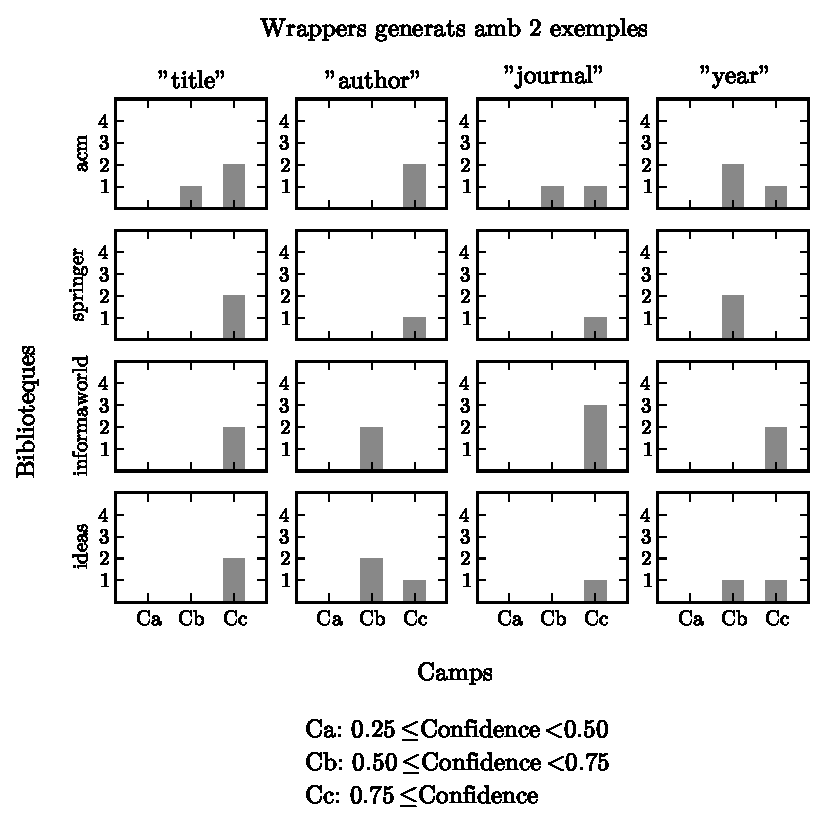
\includegraphics[width=0.8\textwidth]{figures/results:nwrappers-2.pdf}
\caption{Nombre de \textit{Wrappers} generats utilitzant 2 exemples i agrupats per confian�a}
\label{fig:results:nwrappers-2}
\end{center}
\end{figure}


\begin{figure}[H]
\begin{center}
\begin{minipage}{0.49\linewidth}
	\centering
	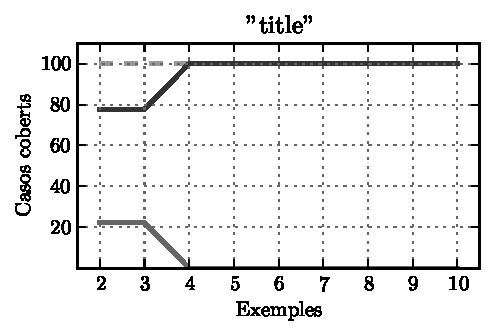
\includegraphics[width=\textwidth]{figures/results:coverage-title.pdf}
\end{minipage}
\hspace{0cm}
\begin{minipage}{0.49\linewidth}
	\centering
	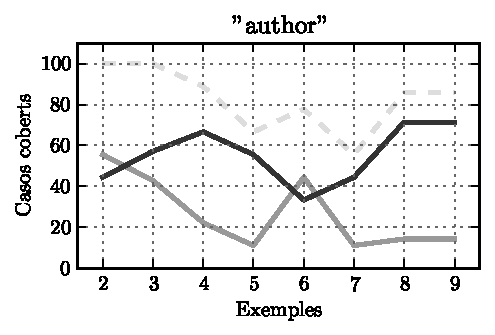
\includegraphics[width=\textwidth]{figures/results:coverage-author.pdf}
\end{minipage}
\end{center}
\end{figure}

\begin{figure}[H]
\begin{center}
\begin{minipage}{0.49\linewidth}
	\centering
	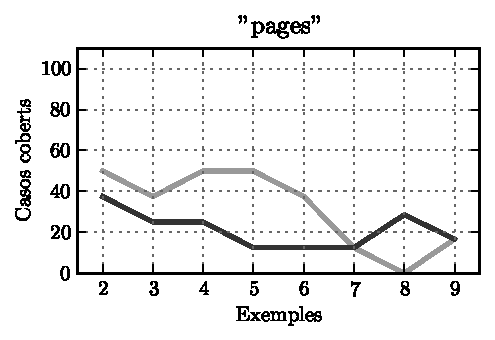
\includegraphics[width=\textwidth]{figures/results:coverage-pages.pdf}
\end{minipage}
\hspace{0cm}
\begin{minipage}{0.49\linewidth}
	\centering
	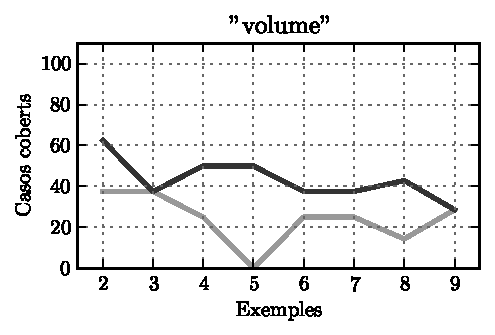
\includegraphics[width=\textwidth]{figures/results:coverage-volume.pdf}
\end{minipage}

\begin{minipage}{\linewidth}
	\centering
	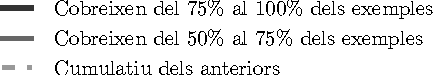
\includegraphics{figures/results:coverage-legend.pdf}
\end{minipage}

\caption{Cobertura dels \textit{wrappers} generats}
\label{fig:appendix:results:wrapperinduction:coverage}
\end{center}
\end{figure}



\begin{figure}[H]
\begin{center}
	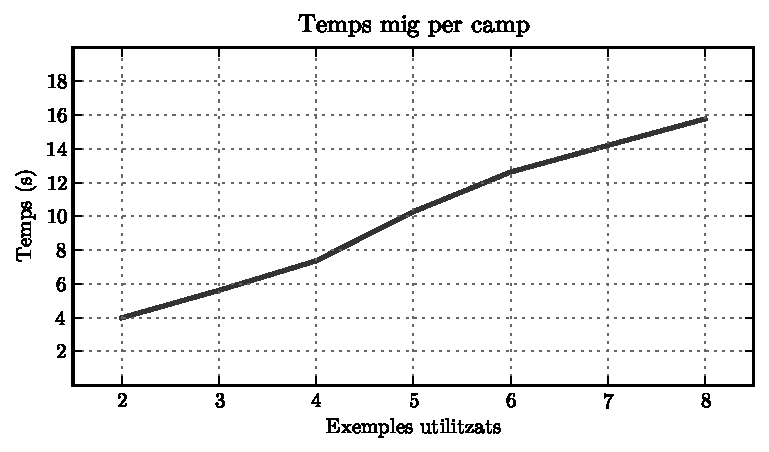
\includegraphics[width=0.8\textwidth]{figures/results:field-time.pdf}
	\caption{Temps mitj� per la generaci� dels \textit{wrappers} d'un �nic camp}
	\label{fig:appendix:results:wrapperinduction:time}
\end{center}
\end{figure}
	




\newpage
\thispagestyle{empty}
\mbox{}

\end{document}
